\documentclass[default]{sn-jnl}
\jyear{2024}%

\theoremstyle{thmstyleone}%
\newtheorem{theorem}{Theorem}
\newtheorem{proposition}[theorem]{Proposition}% 

\theoremstyle{thmstyletwo}%
\newtheorem{example}{Example}%
\newtheorem{remark}{Remark}%

\theoremstyle{thmstylethree}%
\newtheorem{definition}{Definition}%

\raggedbottom

\begin{document}

\title[MGVB tools for proteomics]{\textbf{MGVB: a new proteomics toolset for fast and efficient data analysis}}

\author*[1,2]{\fnm{Metodi V.} \sur{Metodiev}}\email{mmetod@essex.ac.uk}

\affil[1]{\orgdiv{School of Life Sciences, Genomics and Computational Biology Group}, \orgname{University of Essex}, \orgaddress{\street{Wivenhoe Park}, \city{Colchester}, \postcode{CO4 3SQ}, \country{United Kingdom}}}

\abstract{MGVB is a collection of tools for proteomics data analysis. It covers data processing from \textit{in silico} digestion of protein sequences to comprehensive identification of postranslational modifications and solving the protein inference problem. The toolset is developed with efficiency in mind. It enables analysis at a fraction of the resources cost typically required by existing commercial and free tools. MGVB, as it is a native application, is much faster than existing proteomics tools such as MaxQuant and MSFragger and, at the same time, finds very similar, in some cases even larger number of peptides at a chosen level of statistical significance. It implements a probabilistic scoring function to match spectra to sequences, and a novel combinatorial search strategy for finding post-translational modifications, and a Bayesian approach to locate modification sites. This report describes the algorithms behind the tools, presents benchmarking data sets analysis comparing MGVB performance to MaxQuant/Andromeda, and provides step by step instructions for using it in typical analytical scenarios. The toolset is provided free to download and use for academic research and in software projects, but is not open source at the present. It is the intention of the author that it will be made open source in the near future—following rigorous evaluations and feedback from the proteomics research community.  Data used to generate the reported results are available via ProteomeXchange with identifier PXD051331.
}

\keywords{software for computational proteomics, mass spectrometry, MS/MS search engine, shotgun analysis, post-translational modifications}

\maketitle

\section{Introduction}\label{sec1}
Proteomics aims to identify and quantify the proteins expressed in a sample under study at the genome scale (reviewed in \cite{RN1}). At the present the technology of choice—almost universally employed  in large-scale proteomics studies—is high-resolution mass spectrometry of proteolytic digests. Modern hybrid mass spectrometers, when interfaced with nano-scale liquid chromatography, generate many thousands tandem spectra of peptide precursors per run; typical projects often generate more than a million spectra (see for example \cite{RN22, RN23, RN7, RN11} describing the  Orbitrap mass analyser and large-scale proteomics projects that have used it). 

Raw mass spectra are processed by computational pipelines to identify and quantify the proteins. These pipelines utilise search engines that typically match peptide fragmentation spectra to the theoretically predicted sequence specific fragments, i.e. predicted from genomic sequences. Matching is a probabilistic process prone to false positive and false negative results. To account for this, search engines such as Mascot and Andromeda, apply filters, most commonly based on the number of reverse database hits \cite{RN25, RN26}. 

With the advance of instrumentation data processing is becoming the bottleneck of proteomics workflows. To illustrate: practitioners of the art know that at the present a nano-LC-MS/MS experiment will generate 20,000 to 40,000 spectra in an hour or two but MaxQuant  or Mascot or Sequest analysis of the file would take substantial time even on a powerful multicore workstation. In our hands, even when MaxQuant is run under Mono on a high-performance computing cluster, analyses programmed to search for post-translational modifications take longer than the time needed to generate the raw files.

Even more challenging computationally is the recently proposed open search approach, which attempts to identify peptides modified by unknown groups. One implementation of this approach is the MSFragger algorithm \cite {RN3}. It uses precomputed indexed database of peptide fragments to search the MS/MS spectra. MSFragger was publicised as an ultrafast algorithm but it also requires significantly more time to process the data than the hardware needs to generate them. 

Part of the reason for this level of performance is technical: most freely-available search engines are implemented as non native applications running in Java or .Net virtual machines, in part to avoid platform dependence. This puts substantial overheads on memory requirements and execution speed. Another reason is the relative ease of developing in Java and C\#, as they are object oriented garbage-collected languages with rich application libraries ecosystems. However the platform dependence is a less severe problem nowadays as it used to be in the past. A native search engine could potentially provide much faster processing and would come with the added benefit of much smaller carbon footprint as it would use much less memory and processor time. This was the initial motivation behind the MGVB project: to develop a native search engine that could perform as well as the state of the art programs in terms of peptide and protein coverage, but do it faster and with less energy consumption. As it turned out—in the process of development—a new approach to post-translational modification analysis was conceived. It is a combinatorial search that has most of the advantages of the open database search but is much more effective as it is fully capable of handling peptides modified on more that one site and by more than one type of modification, a capability that open search algorithms such as the MSFragger lack by design as they only recognise the total delta mass of the modifications.  This leads to limitations in identifying modified fragment ions when two or more modifications are found on the precursor peptide. This is illustrated in Fig \ref {fig1}.

\begin{figure}[h]
\centering
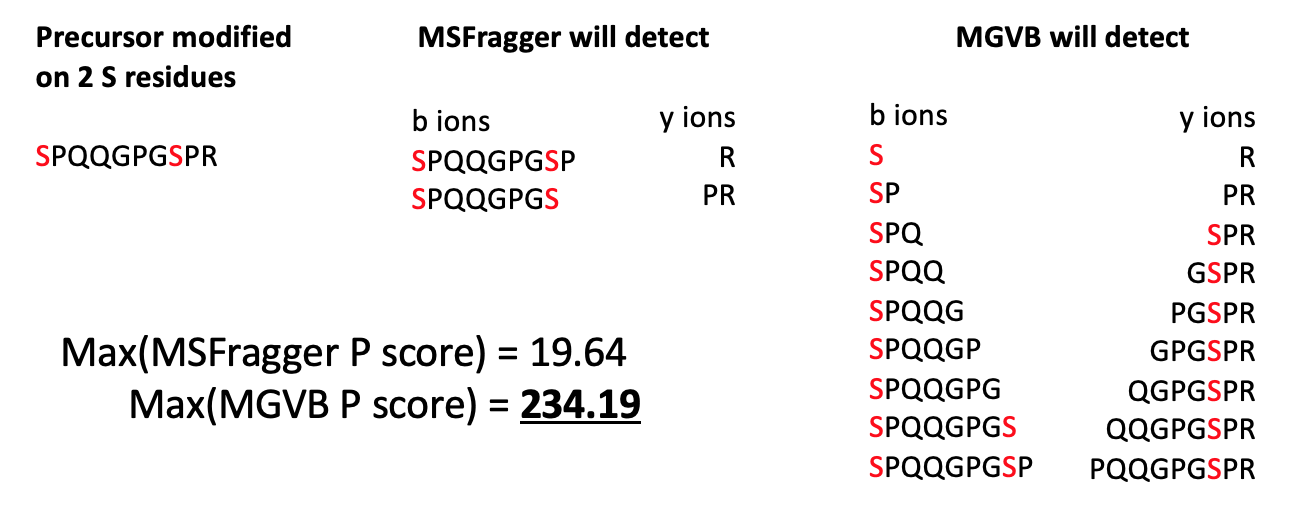
\includegraphics[width=0.9\textwidth]{mgvb_fig1_new.png}
\caption{An example where open database search algorithms would likely fail: two PTMs located near the start and end of the peptide sequence. The combinatorial PTM search algorithm implemented in MGVB can identify y and b fragments and accurately map modification sites in cases where 2 or more residues are modified. Existing open database search engines such as MSFragger cannot do this as they only recognise either unmodified fragment ions or fragment ions that carry all modifications. As a consequence the maximum score that can be achieved by MSFragger would be more than 10 times smaller than the one assigned by MGVB. The match would then likely lose the competition with alternative candidates and will not be reported by MSFragger while MGVB will report it as top candidate. The P scores presented in the figure were calculated assuming q = 5. The score for MSFragger was calculated assuming 4 out of 18 fragment ions were detected. The score for MGVB was calculated assuming 18 out of 18 ions were detected.}\label{fig1}
\end{figure}

MGVB consists of several programs, which prepare peptide sequences, extract raw spectral data to proprietary binary files, match spectra, infer proteins and compute spectral counts to quantify the identified proteins. The \verb scorer  program implements probabilistic algorithms for spectra assignment to sequences, similar to MaxQuant/Andromeda \cite {RN26}. To speed up modified peptides identification, for each candidate precursor sequence, predicted fragments are packaged in a balanced binary search tree, which is used for matching the spectral peaks. A binomial probability score is assigned based on the number of fragments matched. Modifications sites are determined by a Bayesian updating algorithm, which considers assigned fragments as experimental evidences of possible PTM localisation models to compute the final posterior probabilities of localisation. \verb Scorer  outputs results to a text file with extension \verb *.raw.ms2.txt . The file contains information about the top and the second best matches including number of fragments matched, score, retention time, proteins corresponding to the matched spectrum, precursor mass and more.

The combinatorial search algorithm, named \verb scorer_mpi , uses a precomputed database of combinations of up to 3 different post-translational modifications masses called \verb mod_comb . The current compilation of \verb mod_comb  consists of 1394 triplet combinations of 30 different modifications from the Unimod database (Unimod is accessible at \url {http://www.unimod.org}). \verb Scorer_mpi  executes an open database search to identify a set of candidate precursors. It then calculate the delta mass for each of the candidates and searches the mod\_comb database for combinations matching the delta-mass. Once such combination is identified, \verb scorer_mpi  uses the same Bayesian updating algorithm as the \verb scorer  program to accurately determine the location of each modification from the combination. 

A very important advantage of this approach is that only the initial precursor search needs to be restricted to high-mass accuracy. The search for MS/MS fragments matches does not need such accuracy. This makes the huge amount of legacy raw data acquired in the High/Low mode of analysis amenable to processing by \verb scorer_mpi .

\section{Results and Discussion}\label{sec2}

MGVB was tested with a collection of raw data files obtained from experiments with human cell lines. An LTQ/Orbitrap Velos isnstrument was used to generate the data as described in \cite {RN6, RN7, RN9}. The results were obtained by analysing data from immunoprecipitation experiments using GFP-tagged Scribble as bait expressed in human HEK293 cells as described in \cite {RN6}. The performance of MGVB was compared to MaxQuant, version 1.6.1.0 running on the same hardware. 

The following performance metrics were compared: number of MS/MS spectra identified at 1\% FDR (significant PSMs), number of proteins identified at  1\% FDR, number of PTM identified for the target protein Scribble (see below for details of experimental context), speed: time for completing the different steps of the analysis, memory consumption, CPU time. 

The results from these comparisons are summarised in figures \ref {fig2}-\ref {fig3}. Fig. \ref {fig2} shows the peptide and protein identification performance of MGVB compared to MaxQuant/Andromeda. MGVB and MaxQuant find very similar numbers of peptides and proteins at the chosen FDR. However, MGVB assigns more spectra to the bait protein—which is the most abundant protein in the sample by a large margin. Similarly, MGVB assigns slightly more spectra to GFP. The spectral counts for the known Scribble-interacting proteins GIT1 and ARHGEF7 assigned by MGVB and MaxQuant are very similar.  


Fig. \ref {fig3} compares the performance of MGVB and MaxQuant in terms of execution speed, memory consumption and CPU usage. MaxQuant was run under Mono on the same hardware configuration as MGVB. MaxQuant and MGVB were set to search for up to 3 PTMs per peptide and the modifications were set to N-terminal acetylation, methionine oxidation and STY phosphorylation. MGVB outperformed MaxQuant in speed by a large margin and consumed significantly less memory and CPU time per run in all benchmarking experiments. In these experiments MaxQuant was set to not perform second peptide search to make speed comparisons fair. Both search engines conducted first search and precursor mass recalibration followed by a main search.


\begin{figure}[H]
\centering
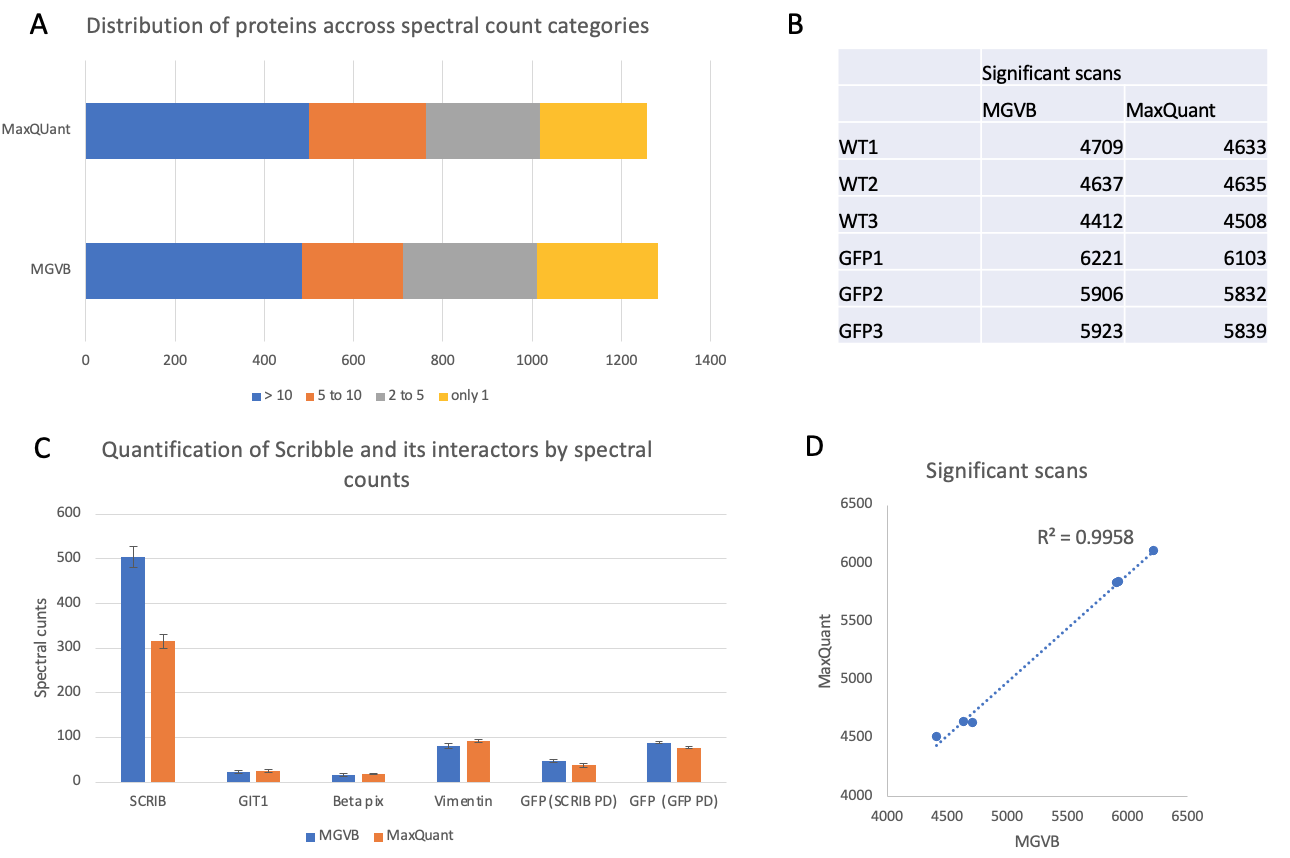
\includegraphics[width=1\textwidth]{mgvb_fig2.png}
\caption{Performance metrics of MGVB compared to MaxQuant. MGVB and MaxQuant were run on the HPC cluster Ceres at University of Essex, UK. Both programs were run on 24-core instances through the grid engine. MaxQuant was run under Mono. Both programs were set to use at most 24 threads: MGVB by setting the environmental variable OMP\_NUM\_THREADS=24; MaxQuant, by setting the number of threads in mqpar.xml. \textbf{A}: number of proteins identified stratified by spectral count ranges. \textbf{B}: number of PSMs passing the FDR filters obtained from the 6 raw files, the numbers of scans assigned from each file were computed by summing up the MS/MS counts from proteinGroups.txt (MaxQuant) and consolidated\_results.txt (MGVB); \textbf{C}: spectral counts assigned to the bait protein Scribble and 4 of its known interacting proteins, and to the negative control bait, GFP; \textbf{D}: correlation plot of the data presented in  \textbf{B}. Error bars represent standard deviation from 3 independent LC-MS/MS runs.}\label{fig2}
\end{figure}


\begin{figure}[h]
\centering
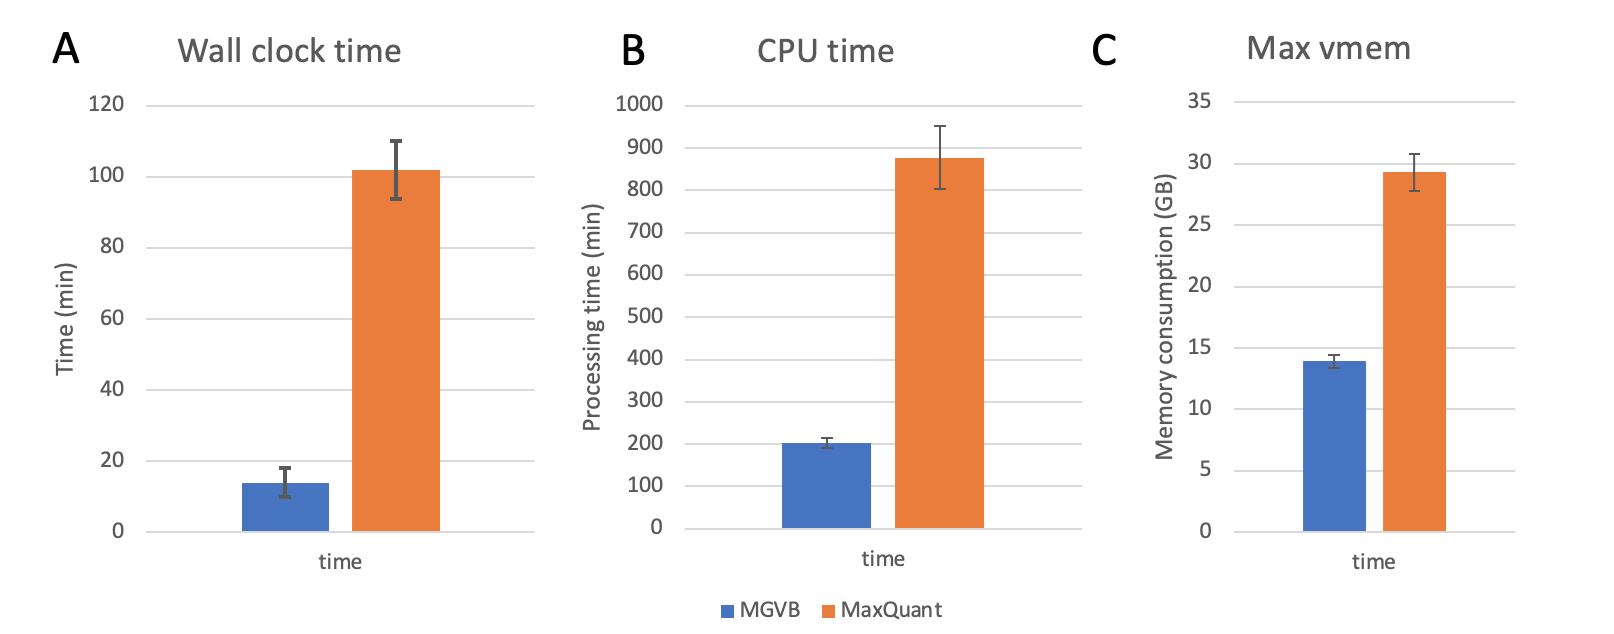
\includegraphics[width=0.9\textwidth]{mgvb_fig3.png}
\caption{Performance metrics of MGVB compared to MaxQuant. MGVB and MaxQuant were run on the HPC cluster Ceres at University of Essex as described in Fig. 2. \textbf{A}: wall clock times for processing 6 raw file;  \textbf{B}: CPU times for the same task;  \textbf{C}: maximum used memory for the same task. Error bars represent standard deviation from 3 independent experiments.}\label{fig3}
\end{figure}

The open search capabilities of MGVB are demonstrated with data in Supplementary Table 1. The table shows that the combinatorial search identifies most known phosphorylation sites of Scribble, as well as known ubiquitination sites and some candidate novel acetylation and methylation sites of potential interest. 

MGVB can perform combinatorial PTM searches to identify pre-selected sets of post-translational modifications in two modes of operation: in an unrestricted mode it searches against the entire genome of the organism under study. This is challenging and requires a high-performance computer. Typically, in such experiments MGVB was run on up to 40 cpus using its inbuilt high-performance message-passing functionality. An alternative mode, the focused search, restricts the analysis to a subset of sequences selected from a preceding ultrafast stringent search. Typically, MGVB was set to initially search without any modification allowed and no missed cleavages. Such searches complete under a minute on a multicore workstation (8 cores). Proteins identified in such searches are then subjected to a focused combinatorial search. Supplementary Table 1 shows that the focused approach correctly identifies most of the phosphorylation sites known for Scribble and suggests several novel modifications. 

Compared to MGVB, recently published open search algorithms such as the one implemented in MSFragger \cite {RN3} suffer from two fundamental limitations. First, they require high mass accuracy for fragment masses. MSFragger, for example, uses a precomputed index of y and b fragment masses which have to be matched with very high mass accuracy. This imposes  strict restriction on the analytical platforms that can be used in the process of generating the data and makes the analysis of legacy high/low data unfeasible. Second, existing open search tools identify candidate peptide modifications by matching the delta mass of the identified peptide to candidate modification in a process that is inherently limited to recognising the modification as a single added group. A lengthy post processing employing machine learning is required to make sense of the initial assignments. For example, a delta mass of W units cannot be immediately assigned to a modification of type A on residue X plus a modification of type B on residue Y because the algorithm has no way of learning what the individual  masses A and B are from their sum. It will report the delta mass and the peptide sequence but it would be up to the researcher to hunt for the identities of A and B. Even more limiting, to the extend of making open search engine unusable for such cases, is the fact that if there are two modification on two different residues, many of the spectral peaks corresponding to y and b fragments will not be assigned by the open search engine (see Fig \ref {fig1} for illustration).

In contrast, MGVB would use the scorer\_mpi module to execute a combinatorial search, which would directly identify the two modifications, A and B, and will localise them to the correct residues—all in a single step analysis. 

An added benefit of using MGVB to perform combinatorial PTM searches is speed of analysis. A typical focused search for combinations of up to 3 PTMs from a list of 30 different modifications completes under 25 min on a 24-core instance. In comparison, an open database search by MSFragger would take several hours.

\section{Methods}\label{sec3}

This section describes the implementation and the algorithms used in MGVB. 

\subsection{Implementation}\label{subsec1}
With a single exception, MGVB is implemented in C and compiled in a collection of binary executable files, which can be used on hardware running the Linux operating system. The one exception, the program used to extract spectra from the proprietary raw files is implemented in C\# in order to leverage the API provided by Thermo Fisher Scientific, but availability of .Net is not required to run it as the program is packaged into an executable file. Table \ref{table1} lists the different programs, and gives brief description of their utility. 

The following external libraries were used to develop MGVB: the arbitrary precision number library MPFR from GNU \cite {RN666}; OpenMP (for shared memory parallelism) \cite {RN667}; Open MPI (for message-passing parallelism) \cite {mpi40}; sqlite3 (for storing and querying data) \cite {sqlite2020hipp}; GNU Scientific Library (for fitting linear models with interaction terms for precursor mass recalibration) \cite {gough2009gnu}. 

\begin{table}[h]
\begin{center}
\begin{minipage}{550pt}
\caption{List of MGVB modules}
\label{table1}
\begin{tabular}{@{}llll@{}}
\toprule
Name  & Description\\
\midrule
\verb digest_universal  & In silico digestion of sequences from FASTA files.\\
\verb mod_pep   & Generate modified peptides sequences.\\
\verb toSQL  & Create sqlite tables with sequences from FASTA files.\\
\verb extractRaw  & Extracts from raw files and writes MS2 and MS1 files to disk\footnotemark[1].   \\
\verb parseMS   & Parses MS2 files to proprietary binary mms files.  \\
\verb scorer   & Uses mms files to search for peptide matches\footnotemark[2].  \\
\verb scorer_mpi  & Uses mms and two sqlite databases to search for PTM\footnotemark[3]. \\
\verb deep_seq  & Prepares sequences for combinatorial PTM search. \\
\verb select_by_pep  & Prepares data for applying the local FDR filtering.\\
\verb create_aggregated  & Generate combined statistics for filtering.\\
\verb select_sig  & Filters candidate peptides using the local FDR approach.\\
\verb select_by_pep_open  & Used for data generated by \verb scorer_mpi .\\
\verb mgvb  & Consolidates results for multiple samples.\\
\botrule
\end{tabular}
\footnotetext[1]{MS1 and MS2 files are text files that can be used by various proteomics search engines \cite {RN27}.}
\footnotetext[2]{Uses the OpenMP library for shared memory parallel processing.}
\footnotetext[3]{Uses the Open MPI library for message passing parallel computations.}
\end{minipage}
\end{center}
\end{table}

In addition to the binary files included in Table \ref {table1}, there is a collection of shell scripts, which automate the various modes of analysis possible with MGVB. These are described in Appendix A.

Running the MGVB pipeline using the provided shell scripts will create numerous files on the host computer. Many of the files contain intermediate information and can be deleted after the project is complete. There are MS1 and MS2 files, which are human readable files with MS and MS/MS scan information closely following the format that is used by RawConverter \cite {RN27}. The mms files are binary files containing the same information. The db files are sqlite database files used to generate the final report. They contain all peptide and protein level data obtained in the course of analysis.

\subsection{Outline of algorithms}\label{subsec2}
The detailed description of the scoring algorithm implemented in the \verb scorer  and \verb scorer_mpi  programs is not provided as it closely follows the published Andromeda scoring algorithm: the same binomial score and the same approach of filtering the top q spectral peaks as MaxQuant/Andromeda are used. 

Where MGVB differs is the algorithm for PTM localisation. Andromeda uses a mapping algorithm that is similar to the one used to match spectra to sequences \cite {RN26}. A binomial probability derived score is computed for each possible PTM assignment model and models with scores above a preselected threshold are selected. 

MGVB departs from this approach and uses a simple Bayesian updating algorithm to assign localisation probabilities. The process starts with generation of all possible PTM localisation models, which are encoded as binary arrays. These are assigned equal prior probabilities. These priors are then updated using the detected fragments as experimental evidences to obtain the posterior probabilities of localisation. 

The Bayesian updating algorithm is described in Algorithm \ref{algorithm1}. MGVB assumes a likelihood of 0.7 if a fragment is compatible with a localisation model and likelihood of 0.2 if not (the likelihood is the probability that the fragment will be observed given that the model in question is true).

\begin{algorithm}
\caption{Calculate PTM localisation models probabilities}\label{algorithm1}\label{algorithm1}
\begin{algorithmic}[1]
\State $models \gets {computeModels}$ \Comment{generates N models}
\State $p \gets {\{\(\frac{1}{N}\), \(\frac{1}{N}\)...\(\frac{1}{N}\)}\}$ \Comment {assigns uniform prior}
\State $F \gets \text{masses of matched fragments in spectrum}$
\ForAll{$f$ in $F$}
        \ForAll{$m$ in $models$}
            \If{$f$, $m$ are compatible}
                \State $p_m \gets p_m \times \lambda_1$                \Comment {if compatible, lambda is set to 0.7}
            \Else
                \State $p_m \gets p_m \times \lambda_0$                \Comment {if not compatible it is usually 0.2}
            \EndIf            
        \EndFor
\EndFor
\State {Renormalise $p$ to sum to 1} 
\end{algorithmic}
\end{algorithm}

The combinatorial PTM search algorithm implemented by \verb scorer_mpi  is presented in Algorithm \ref{algorithm2}. It uses a precompiled database of combinations of up to 3 different PTMs and in its present version covers 30 different modifications derived from Unimod.

The three modules, \verb select_by_pep , \verb create_aggregated , and \verb select_sig  (see Table \ref {table1}) work as a filter pipeline to select peptide hits based on decoy database hits. The filtering pipeline computes the local false discovery rate (also known as posterior error probability, or PEP, see \cite {RN28} for details of how PEP is computed) using all data available as baseline for calculating the parameters of a bivariate Gaussian distribution. As in MaxQuant the two variables are the binomial probability score and the length of the peptide sequence. The Gaussian is then used to compute PEP,  and results are filtered to 1\% FDR  using PEP. 

Algorithm \ref{algorithm1} calculates posterior probabilities for the possible PTM localisation models. Model probabilities p\textsubscript{j} are then converted to site probabilities P\textsubscript{i} using the following equations:

\begin{equation}
{P_i} = \sum\limits_{j=1}^{N}{p}_j \times \gamma_j^i .\label{eq1}
\end{equation}
where,
\begin{align}
\gamma_j^i = 
\begin{cases}
  1 & \text{if site i is modified under model j} \\
  0 & \text{otherwise}
\end{cases}
\end{align}


\begin{algorithm}
\caption{Combinatorial PTM search implemented by scorer\_mpi}\label{algorithm2}
\begin{algorithmic}[1]
\State $mod\_comb \gets \text {generate mod\_comb}$ \Comment{generates delta mass db}
\State $peptides \gets \text {generate peptide db}$ \Comment {generates peptides db}
\ForAll {$s$ in mms file}    \Comment {mms file contains spectra}
       \State $M \gets \text {$peptides$ matching parent of $s$}$    \Comment {usually \textpm 500 Da }
       \ForAll{$m$ in $M$}
           \State $\delta \gets \text {compute delta mass for $m$}$          
           \State $ptm \gets \text {PTM combinations from $mod\_comb$ matching } \delta$
            \ForAll {$c$ in $ptm$}
               \State $score \gets \text {score $s$ against $m$ modified by $c$, save to results}$
            \EndFor            
        \EndFor
\EndFor
\end{algorithmic}
\end{algorithm}




For combinatorial PTM data the algorithm is changed to implement a hybrid approach to optimising FDR: the raw binomial probability score is still used but an additional threshold is calculated as in the Mascot algorithm, which is \(-log_{10}(0.01/n\_seq)\) where n\_seq is the number of candidate sequences. Candidates that have scores below the threshold are filtered out. The filtering then proceeds to compute PEP as above and filter at 1\% FDR using the PEP values. This is implemented in \verb select_by_pep_open .

Algorithm \ref{algorithm3} solves the protein inference problem: given a set of matched peptides passing the score thresholds, what is the optimal peptides to proteins assignment? This is not a trivial problem as many proteins encoded by distinct genes share sequence similarities, which cause peptides to be shared across groups of proteins. MGVB solves the protein inference problem by implementing a recursive algorithm, which assigns peptides to the protein with the highest protein score in the protein group that share these peptides. Two data structures are involved: a linked list of protein groups, each node containing a list of identities of the proteins in the group,  count of spectra matching the group, and a pointer to the next element of the list. In addition, an array of protein data structures is used. This array is sorted by protein score to allow efficient searching.

\begin{algorithm}
\caption{Recursive protein inference from peptide matches}\label{algorithm3}
\begin{algorithmic}[1]
\State $pr\_groups \gets \text {generate linked list of protein\_group structs}$ 
\State $proteins \gets \text {generate sorted array of tuples of protein IDs with scores}$ 
\Function {process\_prot\_groups}{$pr\_groups$, $proteins$}
    \If {$pr\_groups$ is empty}
        \State $return$
    \EndIf
    \State $names \gets \text {split protein IDs in first node of $pr\_groups$ into array} $
    \State $Pr \gets \text {the element of $names$ with the highest score in $proteins$}$
    \State \text {delete all $pr\_groups$ nodes containing $Pr$ summing their counts to $c$}
    \State \text {save $Pr$, $c$ to results}
    \State \text {$return$ $PROCESS\_PROT\_GROUPS$($pr\_groups$, $proteins$)}     
 \EndFunction
 \State \text {$PROCESS\_PROT\_GROUPS$($pr\_groups$, $proteins$)}
\end{algorithmic}
\end{algorithm}
\bigskip

Algorithm \ref{algorithm3} outputs to a file containing spectral counts and protein IDs. MGVB also contains facilities for combining such files into an aggregated report file of comma separated values, which can be further analysed in R, Python, Excel or any other environment for machine learning and statistical analysis. In addition, MGVB creates sqlite database files for each raw file analysed, which contain plethora of information about scans, peptides, modification etc. These can be analysed by sqlite functions or other software operating on SQL databases. Some simple but useful report functions are given in Appendix A.

\section {Concluding remarks} \label {sec4}
MGVB is work in progress. It is easy to use, and delivers results comparable, if not even better than existing tools. If what is needed is seamless expression profiling, or PTM analysis of your favourite protein,  or protein interaction analysis, and the user prefers a single command line tool that can be used with minimum effort, it will deliver. It is much faster than the existing platforms and uses less power and memory. 

However, there are still things to be done. MGVB does not implement second peptide search, and the handling of isotopes could be improved. It will be also good to implement ion intensity-based quatification in the future. Perhaps most important, MGVB should implement advanced machine learning algorithms for optimising FDR and should be able to handle isobaric tags and stable-sotope based quantitative workflows. This is all planed and will be implemented in the next, open source edition of MGVB.

\bmhead{Supplementary information}

Supplementary Table 1 contains results from combinatorial search  of post-translational modifications performed on WT1.raw data file as described in Appendix A.2. Supplementary files contain a single MGVB archive file, which can be used to install the toolset and run it, an sqlite3 file, \verb db1_min.db , which is needed to carry out combinatorial searches, and two config files: \verb config.rms  and \verb config_focused.rms , which can be edited to easily set up custom searches.

\bmhead{Acknowledgments}

The author acknowledges financial support from University of Essex (internal grant to acquire the LTQ/Orbitrap Velos instrument). 

\section*{Declarations}

\begin{itemize}
\item No conflict of interest is reported.
\item No ethics approval was necessary.
\item The raw data files used to generate the reported results are available via ProteomeXchange with identifier PXD051331.\
\item The author was solely responsible for developing MGVB and preparing the manuscipt.
\end{itemize}

\begin{appendices}
\section{Concise guide for the MGVB pipeline}\label{secA}

All programs listed in Table \ref {table1} can be run separately. The format of the commands and arguments for each one can be retrieved from the shell scripts \verb mgvb_auto.sh  and \verb mgvb_focused.sh . The user can then write their own script to compose their own pipelines according to specific project needs. For example, it is not always necessary to extract from raw data files. This can be done just once and then the ms2 files can be used to run the analysis. For researchers, who rely on external LC-MS/MS services, it could be possible even to request the raw data be delivered in as ms2 files. Most facilities are familiar with the ms2 format and can do this. Alternatively, ms2 files can be parsed to binary mms files and these then can be used in multiple runs of the pipeline to search for different combinations of PTMs. 

For combinatorial PTM searches, one does not always need to start from scratch. If \verb mgvb_auto.sh  has been already executed, it will be convenient to use the generated mms.txt files and proceed directly to run \verb scorer_mpi . The shell script can be changed accordingly to do this.

\subsection{Differential expression and protein interaction analysis}\label{secA1}
MGVB is distrinuted as a single archive file. Download and expand the file in a convenient location on your system. When placed in this directory and expanded, the archive will create a subdirectory tree containing mgvb/bin. To install the executables and run the pipeline do:
\begin {enumerate}
\item  {Put mgvb/bin to the path:}
\begin{verbatim} 
export PATH=$PATH:[path to mgvb]/bin
\end{verbatim}
\item {Copy raw data files and \verb config.rms  to a new project directory.}
\item {In the project directory, edit \verb config.rms  to set up the analysis. Change only the necessary entries: raw file names, fasta files and experiment names. If not interested in phosphorylations comment out the entry. Make sure precTol and tol are appropriate for the type of data—High/Low or High/High. The config file contains further instructions as comments to each line of code.}
\item {From within the project directory, execute:}
\begin{verbatim}
mgvb_auto.sh
\end{verbatim}
\item {Multiple result files will be generated. For each raw file there will be a \verb *.raw.ms2.mms.txt  file containing the top 2 candidate PSMs for each MS/MS scan. A \verb *.raw.ms2.mms.txt.db  file contains sqlite tables with peptides, proteins, protein groups and significant PSMs. A \verb *.raw.ms2.mms.sig_proteins.txt  file contains spectral counts for significant proteins for each raw file. Finally, the \verb consolidated_results.txt  file contains a table with all significant proteins detected in all raw files with their spectral counts.}
\end {enumerate}

\subsection {Automated focused analysis} \label {subsubsect2}
\begin {enumerate}
\item {Make sure MGVB is installed (executables and *.sh scripts are on the path).}

\item {Start with a clean directory containing \verb *.raw  files, copy \verb db1_min.db  file, \verb config.rms  and \verb config_focused.rms  from mgvb/bin to this directory.}

\item {Edit \verb config.rms  as in Appendix A1.}

\item {Execute:} 
\begin{verbatim}
mgvb_focussed.sh
\end{verbatim}
\end{enumerate}

\subsection {Interrogate results using sqlite3 functionality}
\begin {enumerate}
\item {Open desired file (let's say it is \verb WT1.raw.ms2.mms.txt.db ):}
\begin{verbatim}
sqlite3 WT1.raw.ms2.mms.txt.db
\end{verbatim}
\item{Inside the sqlite program execute the following to get all significant MS/MS scans assigned to a specific protein (let's say it is Scribble, which is encoded by SCRIB and in the significant protein list has id = 921. The significant protein list is in the file that has "\verb sig_proteins " in its extension):}
\begin{verbatim}
select * from sig_scans where Sequence in (select sequence \
from unnested where Protein = "921");
\end{verbatim}
\item {Alternatively, if one wishes to export the results to tab-delimited text file to be processed by Excel, Python or R, open the desired file in sqlite3 and execute:}
\begin{verbatim}
.header on
.separator \t
.output output_file_name.tsv
select * from sig_scans where Sequence in (select sequence \
from unnested where Protein = "921");
\end{verbatim}
\end {enumerate}

\subsection {Addressing common portability issues with Open MPI} 
The combinatorial PTM search engine, \verb scorer_mpi , is provided as a binary file compiled with Open MPI 5 and as an alternative binary compiled with Open MPI 2. This should cover most target platforms. For example, the author routinely uses the former with the MGVB pipeline on a laptop running Ubuntu 20.04 and the later is running on the HPC cluster Ceres under CentOS linux. However, it is possible that users might experience problems with some of the shared libraries required by the Open MPI implementation running on their server. For such cases the MGVB distribution provides an alternative portable \verb scorer_mpi  package, which includes a header file (\verb scmpi.h ), a shared library (\verb libscmpi.so ) and a source code file (\verb scorer_mpi_portable.c ), which can be easily compiled into a binary file to be used in the MGVB pipeline. The following steps will do this. 
\begin {enumerate}
\item {Expand the provided \verb scorer_mpi.tar.gz  archive in the mgvb/bin directory:}
\begin{verbatim}
cd mgvb/bin
tar -xzvf scorer_mpi.tar.gz
\end{verbatim}

\item {Build the binary. This assumes the mgvb/bin is in /home/user directory (replace "user" in the following command with the proper user name):}
\begin{verbatim}
mpicc -std=c99 -L/home/user/mgvb/bin -g scorer_mpi_portable.c \
  -o scorer_mpi_portable -lscmpi -lmpfr -lgmp -ldl -lm
\end{verbatim}

\item {Modify and export  \verb LD_LIBRARY_PATH  variable:}
\begin{verbatim}
export LD_LIBRARY_PATH=/home/user/mgvb/bin:$LD_LIBRARY_PATH
\end{verbatim}

\item {Replace \verb scorer_mpi  with \verb scorer_mpi_portable :}
\begin{verbatim}
mv scorer_mpi scorer_mpi_old
cp scorer_mpi_portable scorer_mpi 
\end{verbatim}
The pipeline is now ready to run.

\end{enumerate}

\end{appendices}

\bibliography{mgvb-112023}% common bib file

\bibliographystyle{sn-basic}
\end{document}
